\documentclass[conference]{IEEEtran}

%Template version as of 6/27/2024

\usepackage{cite}
\usepackage{amsmath,amssymb,amsfonts}
\usepackage{algorithm}
\usepackage{algorithmicx}
\usepackage{algpseudocode}
\usepackage{graphicx}
\usepackage{textcomp}
\usepackage{xcolor}
\usepackage{array}
\usepackage{multirow}
\usepackage[caption=false,font=footnotesize]{subfig}
\newcolumntype{L}[1]{>{\raggedright\arraybackslash}p{#1}}
\def\BibTeX{{\rm B\kern-.05em{\sc i\kern-.025em b}\kern-.08em
		T\kern-.1667em\lower.7ex\hbox{E}\kern-.125emX}}
\begin{document}
	
	\title{Machine Learning 441 Assignment 3: Active Learning in Neural Networks}
	\author{\IEEEauthorblockN{Kellen M\"ossner}
		\IEEEauthorblockA{
			26024284 \\
			26024284@sun.ac.za}
	}
	\maketitle
	
	\begin{abstract}
	
	\end{abstract}
	
	\section{Introduction}
	Active learning is a supervised machine learning approach in which the learning algorithm has a varied degree of control over the input data that the neural network (NN) is trained on. Many active learning techniques follow the general approach of selecting instances for the training set that the NN has some difficulty classifying or predicting. Active learning allows the NN to select the most informative instances from a candidate pool of training instances. This approach has the benefit of potentially reducing the amount of data required to train the NN and subsequently be more computationally efficient.
	
	Traditional passive learning involves training NN models on a fixed subset of training data. The disadvantage of this approach is that it often leads to redundancy in training data and inefficiency in the training process. Active learning proposes to address these issues by dynamically updating the training set to focus on instances that contribute most to improved generalisation performance. This report explores, implements, evaluates and compares the two active learning strategies, uncertainty sampling and sensitivity analysis selective learning algorithm (SASLA) against the traditional passive learning approach for neural networks, applied to both classification and regression tasks of varying complexity.

	This report is based on the implementation provided in \cite{github}, which contains the source code for Assignment 3.

	\section{Background}\label{B}
	\subsection{Active Learning}
	Active learning is the machine learning technique where the algorithm selects the data that it wants to learn from. This is a dynamic training process where the learning algorithm selects data from a candidate training set. The algorithm selects the most informative instances from the pool of training data that are most likely to provide the greatest improvement in model performance. Active learning has the proposed benefit of reducing training times and better generalisation performance. The algorithm selects the training instances to train the NN on, which leads to a potential reduction in the number of observations required to train the model. Improved generalisation is achieved when the selected data contains enough informative observations to correctly model the problem.
	
	Passive learning follows the approach where models are trained once only on randomly sampled labelled data. Active learning, however, is an iterative process where at each step the model is trained on a labelled subset of the available data, then the most informative data from the unlabelled data pool is selected and the model is retrained on the new dataset containing the additional informative observations. This iterative process is repeated until the models performance stabilises, the dataset becomes exhausted or a specified number of iterations are completed.
	
	The two main approaches to active learning, as outlined in \cite{engelbrecht2001}, are: \textit{incremental learning} and \textit{selective learning}. Incremental learning begins training on a subset of the training set and during training selects more subsets at specific intervals to add to the training set. The training set that the model is trained on continues to grow as more subsets are selected from the candidate sets. Once a subset has been selected it is removed from the candidate set. During incremental learning the size of the training set grows and the size of the candidate set shrinks after each iteration of the algorithm. At each selection interval of the selective learning process a new training subset is selected from the original candidate set. In contrast to incremental learning, selective learning does not remove the selected subsets from the candidate set. This allows for all observations to be selected at each selection interval. The currently selected subset is used to train the model until a convergence criteria met, such as the training loss stagnating. Once this criteria is met a new training subset is selected from the candidate set and the model continues to train on this new training dataset. This process is repeated until the model has converged or another stopping criterion has been met.
	
	\subsection{Uncertainty Sampling}
	Uncertainty sampling (US) selects instances for which the current NN is most uncertain how to label \cite{lewis1994sequential}. The instances that the NN is unsure about are the ones that lie close to or on the decision boundary for classification models and instances that have high prediction errors for regression models. The uncertainty for classification models can be measured in several methods. The first approach is to use the conditional entropy:
	$$
	x^*=\arg \max_{x^{(i)} \in \mathcal{U}} -\Sigma_{y\in Y}P_\theta(y \lvert x^{(i)})\log(P_\theta(y \lvert x^{(i)}))
	$$
	where $P_\theta(y \lvert x^{(i)})$ is the probability that instance $x^{(i)}$ has label $y$. This approach selects the samples that have the highest entropy. 
	Another approach is to use the least confidence uncertainty:
	$$
	x^*=\arg \max_{x^{(i)} \in \mathcal{U}} (1-\max_{y\in Y}P_\theta(y \lvert x^{(i)}))
	$$
	This approach selects samples where the highest class probability is the lowest.
	The last approach is the margin of confidence sampling:
	$$
	x^*=\arg \min_{x^{(i)} \in \mathcal{U}} (P_\theta(y_m \lvert x^{(i)}) - P_\theta(y_n \lvert x^{(i)}))
	$$
	where, $y_m$ is the most likely label and $y_n$ is the next most likely label for the instance $x^{(i)}$. This last approach measures how uncertain the model is to classify an instance by measuring the margin between the two most likely classes. The smaller the margin is the more uncertain the model is.
	
	Uncertainty sampling for regression is an active learning strategy that selects instances from data that a NN is most uncertain how to predict. Predictive uncertainty for a NN is estimated by using an ensemble of neural networks (Lakshminarayanan et al., 2017). A series of NN regression models are trained with different random parameter initialisations. Each NN generates a prediction for all instances of the unlabelled datasets. The predictions variance across the ensemble of neural networks is used as the measure of regression uncertainty. The instances with the highest predictive variance are chosen for labelling and inclusion into the training set.
	
	Combining uncertainty measures for classification and regression with a pool-based greedy active learning algorithm provides a framework for uncertainty sampling for neural networks. The pool-based greedy active learning algorithm iteratively selects the most uncertain instances and incorporates them into the training set. This process is repeated until some specified stopping criterion is met. This criterion is when a given budget of iterations is exceeded or the NN converges to an optimal solution. The general pool-based active learning algorithm is provided in Algorithm~\ref{alg:pool} which comes from \cite{sharma2017}.
	
	\begin{algorithm}[H]
		\caption{Pool-Based Active Learning}
		\label{alg:pool}
		\begin{algorithmic}[1]
			\State\textbf{Input:} $\mathcal{U}$ -- unlabeled data, $\mathcal{L}$ -- labeled data, $\theta$ -- NN model, $B$ -- budget
			\Repeat
			\ForAll{$\langle x^{(i)}, ? \rangle \in \mathcal{U}$}
			\State compute $uncertainty(x^{(i)}, \theta)$
			\EndFor
			\State pick highest uncertainty $x^{*}$ and query its label $y^{*}$
			\State $\mathcal{L} \gets \mathcal{L} \cup \{\langle x^{*}, y^{*}\rangle\}$
			\State $\mathcal{U} \gets \mathcal{U} \setminus \{\langle x^{*}, y^{*}\rangle\}$
			\State Train $\theta$ on $L$
			\State $B \gets B - 1$
			\Until{$B = 0$}
		\end{algorithmic}
	\end{algorithm}
	
	Where $\langle x^{(i)}, ? \rangle \in \mathcal{U}$ represents the $i$-th unlabelled instance from the unlabelled pool $\mathcal{U}$. The algorithm repeatedly samples the most uncertain instances from the unlabelled pool, updates the training set with the uncertain data, removes the instance from the unlabelled pool and retrains the NN on the new training set.
	
	\subsection{Sensitivity Analysis}
	Sensitivity analysis uses a selective learning approach to continuously select subsets from the original training dataset during training. At each iteration of the selection algorithm, the NN selects the most informative patterns from the candidate training set using the knowledge it has already learned in the training process. One of the key aspects of a select learning algorithm is its ability to decide on what information should be used for training and what information can be overlooked. During the training process, a classification model might become uncertain about a previously correctly classified instance. In this case the selective learning algorithm must be able to identify the instance to add it back to the training subset. The most informative patterns for classification problems are often found near the decision boundaries, referred to as the region of uncertainty.
	
	The sensitivity analysis selective learning algorithm as proposed by (Engelbrecht, 2001), uses sensitivity analysis to select patterns in the region of a decision boundary. The proximity of patters to decision boundaries are evaluated using first order derivatives of the output units with respect to input units. The patterns that are closest to the decision boundary are determined to be the most informative and are chosen for training. Patterns that have little to no effect on the outputs of a NN are uninformative and patterns that have a strong influence on NN outputs are informative. Pattern informativeness is defined as the sensitivity of the output vector from a NN to small changes in the input vector. 
	$$
	\Phi^{(p)} \doteq \lVert\vec{S}_o^{(p)}\lVert
	$$
	denotes the informativeness of pattern $p$, where $\vec{S}_o^{(p)}$ is the output sensitivity vector for pattern $p$ and $\lVert\cdot\lVert$ is any suitable norm. 
	The study from \cite{engelbrecht2001} suggests the maximum norm be used to compute the pattern informativeness.
	$$
	\Phi_\infty^{(p)} = \lVert\vec{S}_o^{(p)}\lVert_\infty = \max_{k=1,...,K}\{|S_{o,k}^{(p)}|\}
	$$
	where $S_{o,k}^{(p)}$ refers to the output sensitivity of a single output unit $o_k$ to changes in the input vector $\vec{z}$.
	
	The output sensitivity vector $\vec{S}_o^{(p)}$ is defined as the norm of the output-input layer sensitivity matrix $S_{oz}^{(p)}$. The norm used to calculate each element $k$ of the output sensitivity vector is the sum-norm.
	$$
	S_{o,k}^{(p)}=\lVert S_{oz}^{(p)}\lVert_1 = \Sigma_{i=1}^I \lvert S_{oz,ki}^{(p)}\lvert
	$$
	Where $I$ is the total number of input units including the bias unit to the hidden layer.
	Assuming that sigmoid activation functions are used in the hidden and output layers, each element $S_{oz,ki}^{(p)}$ of the sensitivity matrix is computed using
	$$
	S_{oz,ki}^{(p)}=(1-o_k^{(p)})o_k^{(p)}\Sigma_{j=1}^Jw_{kj}(1-y_j^{(p)})v_{ji}
	$$
	where $w_{kj}$ is the weight between output unit $o_k$ and hidden unit $y_j$, $v_{ij}$ is the weight between hidden unit $y_j$ and input unit $z_{i}$, $o_k^{(p)}$ is the activation value of the output $o_k$, $y_j^{(p)}$ is the activation of hidden unit $y_j$, and $J$ is the total number of hidden units including a bias unit to the output layer.
	A pattern is considered informative if one or more of the output units are sensitive to small perturbations in the input vector. The larger the value of $\Phi_\infty^{(p)}$ the more informative the pattern is.
	
	The SASLA operator $\mathcal{A}$ is defined as 
	$$
	\mathcal{A}(D_C, \mathcal{F}(D_T;W)) = \{p\in D_C | \Phi_\infty^{(p)}>\Psi(\vec\Phi_\infty)\}
	$$
	where $D_C$ is the candidate training set, $W$ represents the weights of the NN, $\mathcal{F}(D_T;W)$ is the function approximation of the NN which transforms observations from the \textit{I}-dimensional input space to the \textit{K}-dimensional output space, using the training patterns in $D_T$. The vector of $\vec{\Phi}_\infty$ is defined as
	$$
	\vec{\Phi}_\infty = (\Phi_\infty^{(1)},...,\Phi_\infty^{(p)},...,\Phi_\infty^{(P_C)})
	$$
	The function $\Psi$ implements the rule used to select patterns and is defined as
	$$
	\Psi(\vec\Phi_\infty)=(1-\beta)\bar{\Phi}_\infty
	$$
	where $\beta$ is the subset selection constant and $\bar{\Phi}_\infty$ is the average pattern informativeness,
	$$
	\Bar{\Phi}_\infty = \frac{\Sigma_{p=1}^{P_C}\Phi_\infty^{(p)}}{P_C}
	$$
	where $P_C$ is the total number of patterns in the candidate training set $D_C$. Patterns are determined to be informative if their informativeness is some factor larger than the average informativeness over all patterns. The subset selection constant $\beta \in [0, 1]$ is used to control the area around the decision boundary which informative patterns may come from. A larger subset selection constant will allow for more informative patterns to be selected. A conservative choice for the subset selection constant is $\beta=0.9$
	
	The new subset of training data $D_{S_s} = 	\mathcal{A}(D_C, \mathcal{F}_{NN}(D_T;W))$ is selected at each selection interval $\tau_s$. Set the training set $D_T=D_{S_s}$ for the next training interval. 
	
	The general SASLA algorithm is outlined below.
	\begin{enumerate}
		\item Initialise weights and learning parameters. \\
		Initialise the pattern selection constant, $\beta=0.9$ as a conservative choice. \\
		Construct the initial training subset $D_{S_0} = D_C$. \\
		Let the training set $D_T=D_{S_0}$.\\
		\item Repeat until convergence
		\begin{enumerate}
		\item Repeat \\
		Train the NN on the training subset $D_T$ until some termination criterion is met.
		\item Compute the new training subset $D_{S_s}$ for the next subset selection interval $\tau_s$:
		\begin{enumerate}
		\item For each $p\in D_C$, compute the sensitivity matrix $S_{oz,ki}^{(p)}$ using the equation for sigmoid activation functions.
		\item Compute the output sensitivity vector $\vec{S}_o^{(p)}$ for each $p\in D_C$.
		\item Compute the informativeness $\Phi^{(p)}$ of each pattern $p\in D_C$
		\item Compute the average pattern informativeness $\bar{\Phi}_\infty$.
		\item Apply the operator $\mathcal{A}(D_C, \mathcal{F}_{NN}(D_T;W))$ to find the subset $D_{S_s}$ of most informative patterns. Then, let $D_T=D_{S_s}$.
		\end{enumerate}
		\end{enumerate}
	\end{enumerate}
	The convergence criterion that could be considered are: maximum number of epochs reached; mean squared error (MSE) is lower than a specified threshold or when the percentage of correctly classified observations reaches a specified threshold.
	
	\section{Implementation}\label{I}
	
	\subsection{Neural Network}
	The neural network for the classification and regression problems was implemented in Python using the PyTorch library~\cite{paszke2019pytorch}. The architecture of the NN consists of the input layer, one hidden layer and one output layer. The sigmoid activation function was applied to the hidden and output layers in the NN. The number of units chosen for the hidden layer was obtained by overestimating the optimal number of hidden units. The number of units in the output layer is dependent on the problem that the NN is solving. A NN for regression problems will consist of a single unit in the output layer whereas for classification problems with one-hot encoded labels, the number of units in the output layer corresponds to the number of classes in the classification problem. Applying the sigmoid activation function to each node in the output layer of classification problems produces a probability for an input belonging to the class corresponding to the output unit. The class label corresponding to the output unit with the highest probability is assigned to the input instance. The loss function and optimisation algorithm used in the NN architecture is the MSE loss and stochastic gradient descent (SGD) optimisation algorithm. For classification with one-hot encoded labels, the MSE loss is computed for each instance as the average of sum of the squared differences between the network outputs and the corresponding elements of the one-hot vector of the true label. The parameters of the SGD algorithm include the learning rate which controls the step size of weight updates, the momentum term which smooths oscillations in the loss function landscape and accelerates convergence, and the weight decay regularisation parameter. Weight decay is a regularisation technique that prevents overfitting by adding a penalty term to the loss function based on the sum of the squared weights of the model. The loss function with weight decay regularisation takes the general form of:
	$$
	Loss(\boldsymbol{\theta}) = MSE(\boldsymbol{\theta}) + \lambda\lVert\boldsymbol{\theta}\lVert_2^2
	$$
	Where $\boldsymbol{\theta}$ is the vector of the model's weights, $\lambda\lVert\boldsymbol{\theta}\lVert_2^2=\Sigma_{i}\boldsymbol{\theta}_i^2$ and $\lambda > 0$ is the weight decay parameter which determines the regularisation strength. Weight decay regularisation penalizes large weights and pushes them towards zero. This manipulates the optimisation algorithm to prefer smaller weights that are more evenly distributed. The weight decay parameter $\lambda$ is problem dependent and requires cross validated hyper parameter tuning to determine the optimal value. The NN was trained on sequential batches of the training data for each epoch or iteration of the training algorithm. Each batch was randomly selected from the full set of training data. The validation set was used to calculate the validation loss for each epoch. 
	
	\subsection{Passive Learning}
	The training algorithm for the passive learning (PL) approach involves training the NN on the entire training dataset for a fixed set of epochs. At the beginning of each epoch the training data is randomly shuffled and the model is updated on sequential batches from the training data. For each batch, the loss is computed, backpropogation is performed and the NN model weights are updated using the SGD optimisation algorithm. Once the training epochs have been exhausted the final trained NN model is returned along with the models training history for the training and validation losses for each epoch.
	
	A pipeline for the passive learning approach was implemented to train the NN for each problem type. The parameters for the pipeline function consists of the NN hyper parameters and two tuples for the training, validation and test splits for the predictor and response variables. Each dataset is unpacked and then converted into tensor objects in preparation for the NN training algorithm. The input and output dimensions for the NN are determined by the shapes of the training data and labels. Two objects for the MSE loss and SGD optimisation algorithms are initialised and passed as parameters to the NN training algorithm. The NN is trained using the training algorithm and the performance of the trained model is evaluated on the test set. The trained NN, the history and the test performance results are returned by the pipeline function.
	
	\subsection{Uncertainty Sampling}
	The uncertainty sampling approach uses the same training algorithm as the passive learning approach, by training numerous times on the expanding training set of uncertain instances. For each iteration of the uncertainty sampling algorithm a NN is trained on the entire training set. This trained model is then used to determine the instances in the unlabelled candidate pool with the highest classification or prediction uncertainty. The labels for these uncertain instances are then obtained and are added to the labelled training pool for a NN to be trained on in the next iteration of the algorithm. This process is repeated until the budget for the number of iterations of the algorithm is exceeded. 
	
	The conditional entropy uncertainty measure was implemented for instances from the classification problems. An ensemble of NN models was used to calculate the predictive uncertainty for instances from the regression problems. The instances that have the highest predictive ensemble variance are the most uncertain instances. A budget for the uncertainty sampling algorithm was set to 25. The number of instances to sample for each iteration of the algorithm was determined by limiting the maximum number of samples to consider to 80\% of the samples from the training set and dividing this number by 25. The budget and sampling strategy was chosen to prevent the uncertainty sampling algorithm from training on the entire training dataset. The initial NN is trained on a randomly sampled subset from the original training set, which becomes the active training set that uncertain instances are added to. Once the budget has been exceeded the training stops and the performance of the final trained model is evaluated on the test set.
	
	\subsection{SASLA}
	The SASLA approach differs to both the passive learning and uncertainty sampling approaches by adaptively refining the training subset at each epoch by selecting the instances with the highest informativeness from the candidate training set. As the NN trains it learns which instances have the highest sensitivity in the model outputs with respect to the inputs and learns that these instances are more informative. The SASLA algorithm identifies the instances in the dataset that are close to decision boundaries for classification problems and instances that have substantial output variation for regression problems.
	
	In the beginning of the SASLA algorithm, the entire candidate set of training instances is used as the initial training subset. After each epoch of training, sensitivity analysis on the trained model parameters is conducted to determine the instances with the highest informativeness in the candidate training pool. The informativeness is computed by propagating the instance through the network and measuring the magnitude of the gradient of the outputs with respect to the inputs. This captures how strongly small perturbations in the input influence the network outputs. A threshold, determined by the selection constant $\beta$, is applied to select the most informative subset. Instances that have an informativeness greater than $(1-\beta)$ times the average informativeness of the entire candidate set are kept for training in the next epoch. A conservative choice of $\beta=0.9$ was chosen for the selection constant. The SASLA algorithm terminates when either the MSE loss falls below a specified threshold or the maximum number of epochs have been exhausted. The performance of the final trained model is then evaluated on the test set.
	
	\section{Empirical Process}\label{EP}
	\subsection{Data Description and Pre-processing}
	A collection of three classification and three function approximation datasets of varying complexity were collected to evaluate the performance of passive and active learning algorithms. The datasets that were considered for the classification problems are the Breast Cancer Wisconsin Diagnostic dataset \cite{breast}, the Mobile Price Classification dataset \cite{mobile} and the Letter Recognition dataset \cite{letter}. The datasets considered for the function approximation problems were the Boston Housing Prices dataset \cite{boston}, the Concrete Compressive Strength dataset \cite{concrete} and the Abalone Age dataset \cite{abalone}. Each dataset has a varying degree of complexity, observations, features and data quality issues. The datasets and the pre-processing details are described below. After applying the necessary data pre-processing techniques to each dataset, they were split into 70\% training, 10\% validation and 20\% test sets. The split for each classification class was stratified to preserve equal class distribution in the training, validation and test sets. After splitting the data, the numerical input features were scaled to the range $[-1, 1]$ The target feature for the regression problems were scaled to the range $(0, 1)$, which is the output range of the sigmoid activation function. The target features for the classification problems were one-hot encoded into vectors with a one in the $i$-th index indicating that the observation belongs to the $i$-th class. One-hot encoding the target class features allows for sigmoid activation functions on the output nodes and the MSE loss function to be used in training.
	
	\subsubsection{Breast Cancer Wisconsin}
	The Breast Cancer Wisconsin dataset consists of 569 instances with 30 numeric features and one categorical target variable. The categorical target variable contains two classes, M for malignant and B for benign tumours. The categorical target variable was first binary encoded, with 1 representing M and 0 representing B, followed by the one-hot encoding transformation. The class distribution for the target variable is 357 instances belonging to class 0 and 212 instances belonging to class 1. The dataset did not consist of any missing values.
	
	\subsubsection{Mobile Price Classification}
	The Mobile Price Classification dataset consists of 3000 instances with 20 numeric features and one categorical target variable. The categorical target variable
	contains four classes indicating the price range for mobile phones. The classes for the price ranges consist of 0 (low cost), 1 (medium cost), 2 (high cost) and 3 (very high cost). The target variables was transformed into a one-hot encoded vector representation. The class distributions for the target variable is 993 instances belonging to class 0, 1,007 instances belonging to class 1, 500 instances belonging to class 2 and 500 instances belong to class 3. The class imbalances were retained to increase the complexity of the classification problem. The dataset did not consist of any missing values.
	
	\subsubsection{Letter Recognition}
	The Letter Recognition dataset consists of 20,000 instances with 16 numeric features and one categorical target variable. The categorical target variable consists of 26 classes, each representing a letter of the alphabet. The target variable was encoded into numeric class labels before transforming the target into a one-hot encoded vector representation. The class distributions for the target variable ranges from 734 to 813 instances per class. The dataset did not consist of any missing values.
	
	\subsubsection{Boston Housing Prices}
	The Boston Housing Prices dataset consists of 506 instances with 13 numeric features one regression target variable. The target variable contains the median housing price value in the are of Boston. The dataset contained 3.95\% missing values across certain features. These missing values were imputed with the average values for the features. The target variable was scaled to the range $(0, 1)$, to match the output range of the sigmoid activation function.
	
	\subsubsection{Concrete Compressive Strength}
	The Concrete Compressive Strength dataset consists of 1,030 instances with eight numeric features and one regression target variable. The target variable contains the compressive strength of concrete, measured in megapascals. The target variable was scaled to the range $(0, 1)$. The dataset did not consist of any missing values.
	
	\subsubsection{Abalone Age}
	The Abalone Age dataset consists of 4,177 instances with seven numeric features, one categorical feature and one regression target variable. The target variable contains the age of abalones, which is determined by cutting the abalone's shell through a cone, staining it, and counting the number of rings through a microscope. The categorical \texttt{Sex} feature of the dataset was transformed into a one-hot encoded vector representation. The target variable was scaled to the range $(0, 1)$. The dataset did not consist of any missing values.
	
	\subsection{Hyper Parameter Tuning}
	A NN requires an optimal set of hyper parameter values in order to obtain the best performance of the model. These hyper parameters are problem dependent and require extensive tuning in order to determine the optimal values. A grid search cross validation approach was implemented to determine these optimal values. The parameters were searched over a grid of possible values and the results for each parameter combination were evaluated with 5-fold cross validation. The values with the best mean cross validation scores were selected as the optimal set of hyper parameters. The F1 scores from the classification problems and the R-squared scores from the regression problems were used as the cross validation scores. The grid of hyper parameters that required tuning is listed below:
	\begin{itemize}
		\item \texttt{n\_epochs}: the number of epochs that the NN is trained for.
		\item \texttt{batch\_size}: the size of the batches of data trained per each epoch.
		\item \texttt{learning\_rate}: the learning rate for the SGD algorithm.
		\item \texttt{momentum}: the momentum parameter for the SGD algorithm.
		\item \texttt{weight\_decay}: the $\lambda$ parameter for the weight decay regularisation approach.
	\end{itemize}
	Table~\ref{tab:hyperparameters} lists the NN architecture and the hyper parameters that were obtained for each problem from the grid search cross validation algorithm. These hyper parameter values were used with the passive learning, uncertainty sampling and SASLA algorithms as described in Section~\ref{I} to train the NN models for each classification and regression problem.
	\begin{table*}[!t]
		\centering
		\caption{The hyper parameters for passive learning, uncertainty sampling and SASLA experiments}
		\label{tab:hyperparameters}
		\begin{tabular}{L{3cm}L{1.8cm}L{2.5cm}L{1.5cm}L{1.5cm}L{1.5cm}L{1.5cm}L{1.5cm}}
			\hline
			\textbf{Problem} & \textbf{NN Architecture} & \textbf{Train/ Validation/ Test Split} & \textbf{Number of Epochs} & \textbf{Batch Size} & \textbf{Learning Rate} & \textbf{Momentum} & \textbf{Weight Decay $\lambda$} \\
			\hline
			\textit{Breast Cancer Wisconsin} & 30-16-2 & 398/57/114 & 500 & 32 & 0.1 & 0.8 & 0.0001 \\
			\textit{Mobile Price Classification} & 20-12-4 & 2100/300/600 & 200 & 16 & 0.1 & 0.9 & 0.00001 \\
			\textit{Letter Recognition} & 16-24-26 & 14000/2000/4000 & 1000 & 32 & 0.5 & 0.9 & 0.00001 \\
			\textit{Boston Housing Prices} & 13-12-1 & 353/51/102 & 500 & 16 & 0.5 & 0.8 & 0.00001 \\
			\textit{Concrete Compressive Strength} & 8-8-1 & 721/103/206 & 500 & 16 & 0.5 & 0.8 & 0.00001 \\
			\textit{Abalone Age} & 9-16-1 & 2923/418/836 & 500 & 16 & 0.05 & 0.9 & 0.00001 \\ 
			\hline
		\end{tabular}
	\end{table*}
	
	\subsection{Performance Metrics}
	The performances for each NN model was evaluated using the test set. The performance metrics that were considered for the classification problems were accuracy, precision, recall and F1 score. The accuracy measures how often the model's predictions are correct overall however this metric is misleading for imbalanced datasets. The precision measures how many of instances predicted to one class actually belong to that class, and recall measures how many of the actual instances of that class were correctly identified by the model. The F1 score is the harmonic mean between the precision and recall metrics to balance their trade-off.
	
	The performance metrics considered for the regression problems were the mean squared error (MSE), root mean squared error (RMSE), mean absolute error (MAE) and the R-squared value. The MSE calculates the average of the squared differences between predicted and actual values, where larger errors are penalize heavily by the squaring function. The RMSE is the square root of MSE, providing an error metric in the same units as the target variable. The MAE measures the average absolute value of the difference between predictions and actual values, and is more robust to outliers. The R-squared value indicates the proportion of variance in the dependent variable that is explained by the NN. The R-squared value ranges from 0 to 1, with values closer to 1 indicating a better model fit and predictive power.
	
	The results for each training algorithm, passive learning, uncertainty sampling and SASLA, were recorded over multiple independent training runs. Ten independent NN models were trained for each learning approach and each problem dataset. The results from these independent runs were recorded and the averages of these results were used for the non-parametric statistical comparison tests and ranking approaches. The number of independent runs was selected to balance computational cost with the normality assumption, ensuring an accurate comparison of the means.
	
	\subsection{Statistical Tests}
	The non-parametric statistical comparison tests were all conducted at an alpha level of $\alpha=0.05$. The Friedman test was used to determine whether a significant difference in the performance of a set of algorithms exists. The F1 scores from the classification problems were used to compare the multiple learning algorithms with the Friedman statistical test. For the regression problems, the R-squared scores were used for the statistical comparison tests. The null and alternative hypotheses for the Friedman test are:
	\begin{itemize}
		\item $H_0$: All algorithms perform equally on average, the median ranks of their performances are the same and any observed differences are due to random variation.
		\item $H_a$: At least one algorithm performs significantly different to the others and not all medians are equal.
	\end{itemize}
	If the null hypothesis is rejected then there is a significant difference between the algorithms. If there is a significant difference then the post-hoc pairwise Wilcoxon signed-rank tests were performed to identify which algorithms were significantly different. The results from the Wilcoxon signed-rank tests along with the average ranks for each algorithm were collected and displayed in critical difference plots.
	
	The number of wins, losses and ties were calculated for each algorithm based on each performance metric. These wins, losses and ties were calculated by conducting a systematic pairwise comparison using paired t-tests. Each active learning method was compared against the passive learning benchmark across all datasets and performance measures. For each dataset the performance values from multiple independent runs were subjected to a paired one-tailed t-test. The outcomes of the tests were classified as follows: A win was assigned if the active learning method was statistically significantly better than the benchmark at a significance level of $\alpha=0.05$; a loss was assigned if the active learning method was significantly worse; and a tie was assigned if there was no statistical significant difference between the two algorithms. This procedure was repeated for all datasets and performance measures, and the counts of each outcomes were aggregated into a final table of performance results.
	
	\section{Results \& Discussion}\label{RD}
	The test results for the classification and regression performance of the passive learning, uncertainty sampling and SASLA algorithms are tabulated in Table~\ref{tab:classification_results} and \ref{tab:regression_results} respectively. These results show the average performances for each algorithm across all datasets. 
	
	The performances of the learning algorithms on the classification datasets do not differ substantially and there was no clear algorithm which consistently performed the best. The results in Table~\ref{tab:classification_results} show that each learning algorithm performed better than the other algorithms for certain datasets according to the average F1 scores. For example, SASLA achieved the best F1 score on the Breast Cancer dataset, while passive learning performed best on the Mobile Price dataset, and uncertainty sampling was superior on the Letter Recognition dataset. This suggests that the benefits of each strategy are dataset-dependent. The highlighted F1 scores represent the highest performing algorithm for each dataset. The uncertainty sampling test results achieved the best stability alongside competitive results when compared against the other approaches. This reinforces uncertainty sampling as a viable strategy for problems with limited data availability. 
	
	\begin{table}[htbp]
		\centering
		\caption{Classification results for each learning strategy}
		\label{tab:classification_results}
		\resizebox{\columnwidth}{!}{%
		\begin{tabular}{llllll}
			\hline
			\textbf{Problem} & & \textbf{Accuracy} & \textbf{Precision} & \textbf{Recall} & \textbf{F1 Score} \\
			\hline
			\multirow{3}{*}{Breast Cancer}
			& PL   & 0.9842 $\pm$ 0.0035 & 1.0000 $\pm$ 0.0000 & 0.9571 $\pm$ 0.0095 & 0.9781 $\pm$ 0.0049\\
			& US & 0.9833 $\pm$ 0.0026 & 1.0000 $\pm$ 0.0000 & 0.9548 $\pm$ 0.0071 & 0.9768 $\pm$ 0.0037 \\
			& SASLA       & 0.9868 $\pm$ 0.0044 & 1.0000 $\pm$ 0.0000 & 0.9643 $\pm$ 0.0119 & \textbf{0.9818 $\pm$ 0.0062}  \\
			\hline
			\multirow{3}{*}{Mobile Price} 
			& PL    & 0.8053 $\pm$ 0.0144 & 0.8483 $\pm$ 0.0156 & 0.8469 $\pm$ 0.0101 & \textbf{0.8461 $\pm$ 0.0132} \\
			& US & 0.8012 $\pm$ 0.0093 & 0.8502 $\pm$ 0.0077 & 0.8444 $\pm$ 0.0075 & 0.8408 $\pm$ 0.0113 \\
			& SASLA       & 0.8055 $\pm$ 0.0103 & 0.8531 $\pm$ 0.0103 & 0.8484 $\pm$ 0.0074 & 0.8457 $\pm$ 0.0095 \\
			\hline
			\multirow{3}{*}{Letter Recognition} 
			& PL     & 0.7567 $\pm$ 0.0029 & 0.7785 $\pm$ 0.0038 & 0.7552 $\pm$ 0.0029 & 0.7530 $\pm$ 0.0034 \\
			& US & 0.7636 $\pm$ 0.0023 & 0.7822 $\pm$ 0.0039 & 0.7623 $\pm$ 0.0023 & \textbf{0.7614 $\pm$ 0.0027} \\
			& SASLA       & 0.7560 $\pm$ 0.0032 & 0.7784 $\pm$ 0.0027 & 0.7545 $\pm$ 0.0032 & 0.7524 $\pm$ 0.0032 \\
			\hline
		\end{tabular}
	}
	\end{table}
	
	Analysing the regression results reveals a similar pattern. No single learning algorithm consistently achieved the best performance across all datasets, as shown in Table~\ref{tab:regression_results}. Passive learning achieved the highest R-squared value on the Boston Housing and Abalone datasets. Uncertainty sampling obtained the best R-squared score on the Concrete Compressive Strength dataset, suggesting that it was better suited for the problem. The SASLA algorithm, while competitive, did not clearly outperform the other methods but maintained a performance that was competitive to the other scores. The uncertainty sampling showed th best stability in results for the two simpler regression problems, while still achieving competitive results. However, the uncertainty sampling algorithm performed the worst on the more complex Abalone Age problem with a much less stable result. This suggests that uncertainty sampling is better suited to simpler regression tasks instead of complex ones. 
	
	\begin{table}[htbp]
		\centering
		\caption{Regression results for each learning strategy}
		\label{tab:regression_results}
		\resizebox{\columnwidth}{!}{%
		\begin{tabular}{llllll}
			\hline
			\textbf{Problem} &  & \textbf{MSE} & \textbf{RMSE} & \textbf{MAE} & \textbf{R-squared} \\
			\hline
			\multirow{3}{*}{Boston Housing}
			& PL    & 0.0062 $\pm$ 0.0004 & 0.0789 $\pm$ 0.0023 & 0.0515 $\pm$ 0.0019 & \textbf{0.8279 $\pm$ 0.0101} \\
			& US & 0.0066 $\pm$ 0.0003 & 0.0813 $\pm$ 0.0019 & 0.0548 $\pm$ 0.0011 & 0.8176 $\pm$ 0.0089 \\
			& SASLA       & 0.0069 $\pm$ 0.0008 & 0.0828 $\pm$ 0.0047 & 0.0564 $\pm$ 0.0050 & 0.8099 $\pm$ 0.0221 \\
			\hline
			\multirow{3}{*}{Concrete Strength} 
			& PL     & 0.0070 $\pm$ 0.0023 & 0.0828 $\pm$ 0.0117 & 0.0641 $\pm$ 0.0091 & 0.8250 $\pm$ 0.0566 \\
			& US & 0.0062 $\pm$ 0.0005 & 0.0784 $\pm$ 0.0029 & 0.0612 $\pm$ 0.0030 & \textbf{0.8461 $\pm$ 0.0117} \\
			& SASLA       & 0.0063 $\pm$ 0.0008 & 0.0792 $\pm$ 0.0048 & 0.0611 $\pm$ 0.0035 & 0.8424 $\pm$ 0.0199 \\
			\hline
			\multirow{3}{*}{Abalone Age} 
			& PL     & 0.0065 $\pm$ 0.0001 & 0.0808 $\pm$ 0.0006 & 0.0589 $\pm$ 0.0010 & \textbf{0.5274 $\pm$ 0.0067} \\
			& US & 0.0071 $\pm$ 0.0004 & 0.0841 $\pm$ 0.0024 & 0.0642 $\pm$ 0.0043 & 0.4869 $\pm$ 0.0292 \\
			& SASLA       & 0.0065 $\pm$ 0.0000 & 0.0808 $\pm$ 0.0003 & 0.0587 $\pm$ 0.0013 & 0.5268 $\pm$ 0.0031 \\
			\hline
		\end{tabular}
	}
	\end{table}
	
	 The boxplots in Figure~\ref{fig:classification_boxplots} and \ref{fig:regression_boxplots} summarizes the performance metrics over the ten independent runs for each learning algorithm. The performance metrics were averaged across each problem dataset. The classification boxplots in Figure~\ref{fig:classification_boxplots} visualise the minor differences between the performances for each learning algorithm on the classification problems datasets.
	 
	\begin{figure}[htbp]
		\centering
		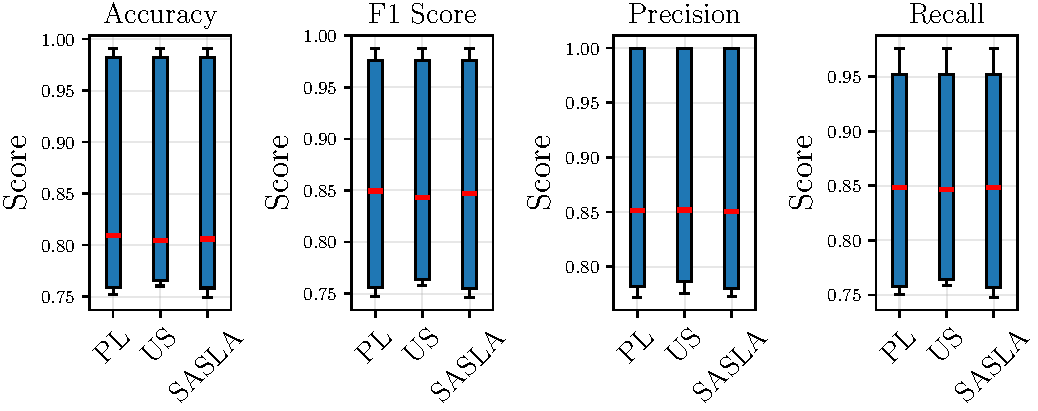
\includegraphics[width=\linewidth]{plots/classification_boxplots.pdf}
		\caption{Classification results boxplots for passive learning, uncertainty sampling and SASLA.}
		\label{fig:classification_boxplots}
	\end{figure}
	
	Noticeable variations across the regression boxplots in Figure~\ref{fig:regression_boxplots} can be seen. The R-squared boxplot for uncertainty sampling has a longer tail than the other learning algorithms, indicating the results for uncertainty sampling contained smaller minimum values. This suggests that the uncertainty sampling algorithm has the potential to perform worse than the other learning algorithms for more complex regression problems.  
	
	\begin{figure}[htbp]
		\centering
		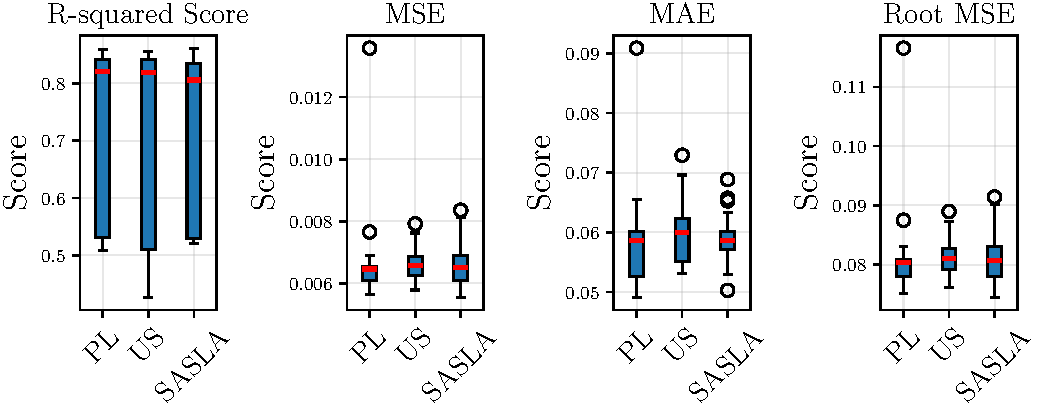
\includegraphics[width=\linewidth]{plots/regression_boxplots.pdf}
		\caption{Regression results boxplots for passive learning, uncertainty sampling and SASLA.}
		\label{fig:regression_boxplots}
	\end{figure}
	
	Figure~\ref{fig:uncertainty_sampling_all} represents the average F1 and R-squared scores for the uncertainty sampling as the size of the training set increases. The average scores and their error bars are plotted at for each sampling interval of the uncertainty sampling algorithm. The blue plots represent the classification problem datasets and the red plots represent the regression problem datasets. A general trend can be seen with the performance scores increases as the size of the training set increases. The plot in Figure~\ref{fig:mp_uncertainty_sampling} stands out as the F1 score initially decreased when the new uncertain instances were added to the training set before and increased after more than 1,000 samples were added to the training set. Figure~\ref{fig:bc_uncertainty_sampling} shows how quickly the uncertainty sampling algorithm converged to a stable F1 score. The algorithm required substantially fewer training instances to achieve a level of performance that is comparable to passive learning and SASLA approaches. This further highlights the advantage computational advantage of uncertainty sampling requiring fewer training instances.
	
	\begin{figure}[htbp]
		\centering
		\subfloat[Breast Cancer Wisconsin]{
			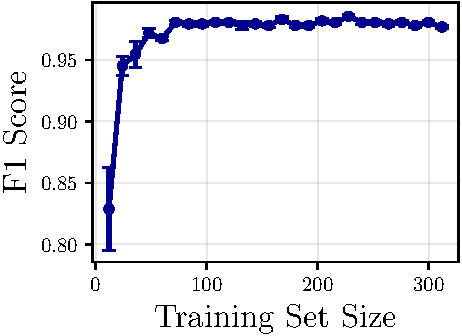
\includegraphics[width=0.45\linewidth]{plots/breast_cancer_uncertainty_sampling.pdf}
			\label{fig:bc_uncertainty_sampling}
		}
		\hfil
		\subfloat[Mobile Price Classification]{
			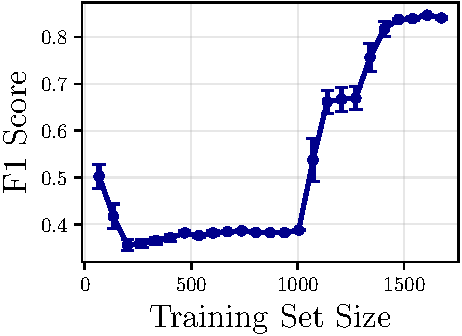
\includegraphics[width=0.45\linewidth]{plots/mobile_pricing_uncertainty_sampling.pdf}
			\label{fig:mp_uncertainty_sampling}
		}
		
		\subfloat[Letter Recognition]{
			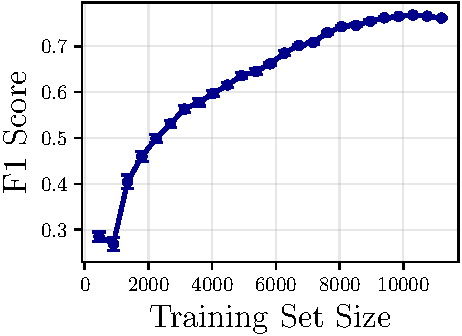
\includegraphics[width=0.45\linewidth]{plots/letter_recognition_uncertainty_sampling.pdf}
			\label{fig:lr_uncertainty_sampling}
		}
		\hfil
		\subfloat[Boston Housing]{
			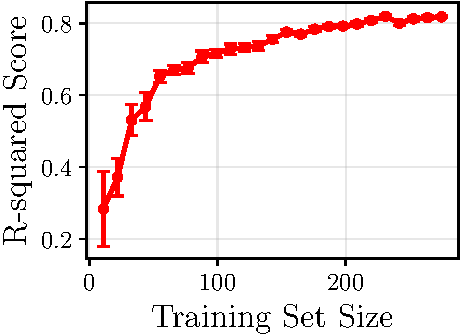
\includegraphics[width=0.45\linewidth]{plots/boston_housing_uncertainty_sampling.pdf}
			\label{fig:bh_uncertainty_sampling}
		}
		
		\subfloat[Concrete Compressive Strength]{
			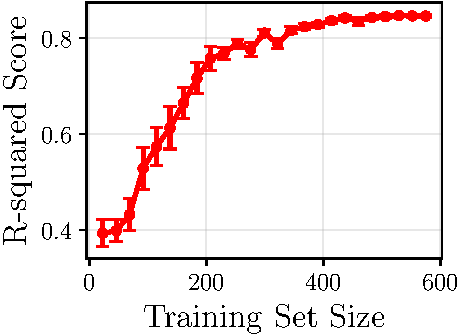
\includegraphics[width=0.45\linewidth]{plots/concrete_strength_uncertainty_sampling.pdf}
			\label{fig:ccs_uncertainty_sampling}
		}
		\hfil
		\subfloat[Abalone Age Prediction]{
			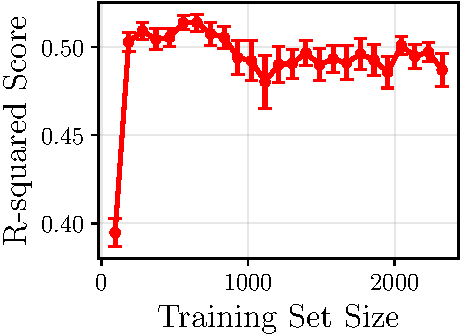
\includegraphics[width=0.45\linewidth]{plots/abalone_age_uncertainty_sampling.pdf}
			\label{fig:aa_uncertainty_sampling}
		}
		\caption{The uncertainty sampling performance results over time as the training subset increases.}
		\label{fig:uncertainty_sampling_all}
	\end{figure}
	
	The error bars at each selection interval follows a general convergence trend where the average performance scores become more stable as more samples are added to the training set. The results in Figure~\ref{fig:aa_uncertainty_sampling} do not follow this trend which is explained by the complexity of problem. This provides reason to suggest that uncertainty sampling does not perform well for complex regression tasks and should instead be considered for classification tasks where resources such as compute and training data are limited.
	
	Figure~\ref{fig:sasla_selection_all} represents the pattern selection over time for the SASLA algorithm across the six different datasets. Each point in the plots represent the size of the sampled training set from the candidate set that was deemed to have informative patterns by the SASLA selection algorithm. A somewhat general trend can be seen in the plots where the size of the sampled patterns from the candidate set decreases over time for each epoch. This trend however is not consistent among all datasets and some problems sample more data than previous iterations as seen in Figures~\ref{fig:bh_sasla_selection} and \ref{fig:ccs_sasla_selection}. 
	\begin{figure}[htbp]
		\centering
		\subfloat[Breast Cancer Wisconsin]{
			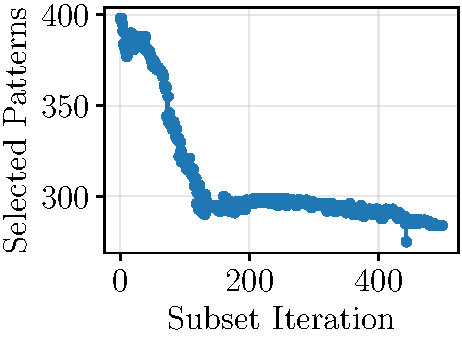
\includegraphics[width=0.45\linewidth]{plots/breast_cancer_sasla_selection.pdf}
			\label{fig:bc_sasla_selection}
		}
		\hfil
		\subfloat[Mobile Price Classification]{
			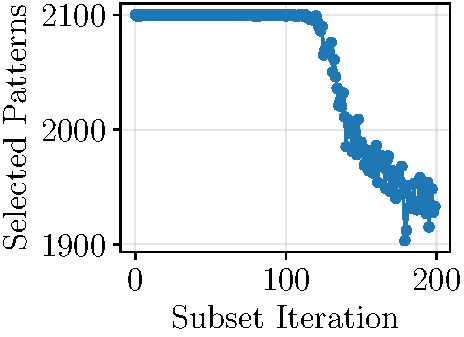
\includegraphics[width=0.45\linewidth]{plots/mobile_pricing_sasla_selection.pdf}
			\label{fig:mp_sasla_selection}
		}
		
		\subfloat[Letter Recognition]{
			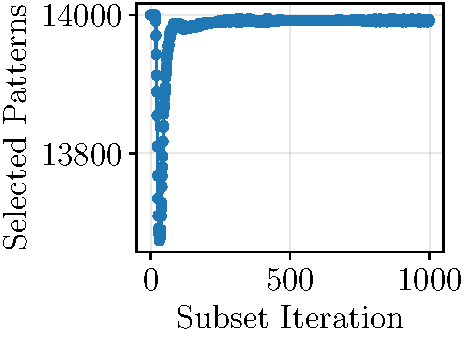
\includegraphics[width=0.45\linewidth]{plots/letter_recognition_sasla_selection.pdf}
			\label{fig:lr_sasla_selection}
		}
		\hfil
		\subfloat[Boston Housing]{
			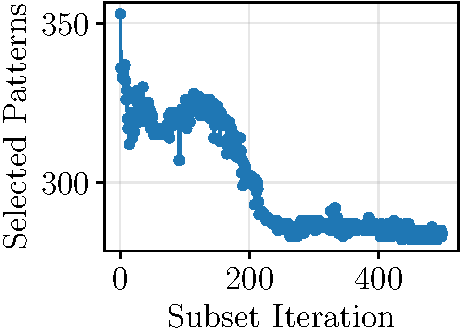
\includegraphics[width=0.45\linewidth]{plots/boston_housing_sasla_selection.pdf}
			\label{fig:bh_sasla_selection}
		}
		
		\subfloat[Concrete Compressive Strength]{
			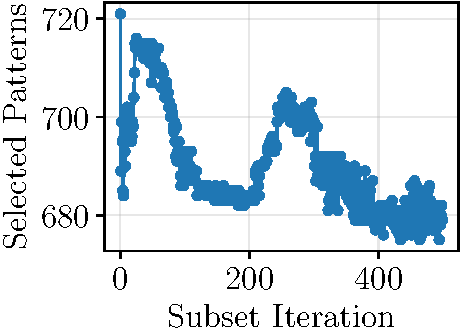
\includegraphics[width=0.45\linewidth]{plots/concrete_strength_sasla_selection.pdf}
			\label{fig:ccs_sasla_selection}
		}
		\hfil
		\subfloat[Abalone Age Prediction]{
			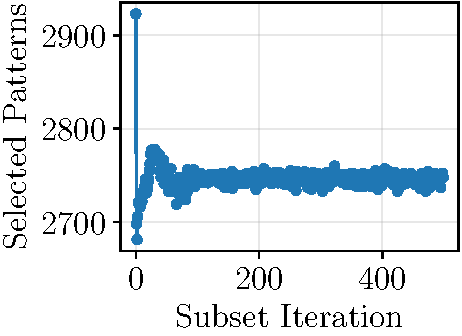
\includegraphics[width=0.45\linewidth]{plots/abalone_age_sasla_selection.pdf}
			\label{fig:aa_sasla_selection}
		}
		\caption{Pattern selection over time by the SASLA algorithm across the six datasets.}
		\label{fig:sasla_selection_all}
	\end{figure}
	
	Another noticeable insight to the SASLA algorithm is that it tended to select fewer patterns for the simpler problems than the more complex problems. The pattern selections for the simple problems, shown in Figures~\ref{fig:bc_sasla_selection} and \ref{fig:bh_sasla_selection}, show an immediate decrease in the number of patterns considered for training. This is a stark contrast to the pattern selection plots in Figures~\ref{fig:lr_sasla_selection} and \ref{fig:aa_sasla_selection} for the complex problems. The number of selected patterns initially decreased before they rapidly increased again and stabilised after a few iterations. This indicates that the SASLA algorithm could not differentiate between uninformative and informative patterns for complex problems. Instead, the SASLA algorithm identified a large portion of the candidate training set as informative, indicating that NN model is unsure about most of the predictions it generates.
	
	The Friedman statistical test for the F1 and R-squared scores of the learning algorithms were conducted at a significance level of $\alpha=0.05$. If the Friedman test identified a significant difference between the algorithms performances then the Nemenyi post-hoc test was performed to identify the significant differences. The results for the Friedman tests for both the classification and regression problem performances had a p-value of $p=0.716531$. This p-value is far greater than the significance level $\alpha$, $0.716531 \gg 0.05$. Therefore, there was no statistically significant difference between the performances of the learning algorithms and the null hypothesis was accepted. 
	
	The critical difference plots for the classification and regression performances are shown in Figures~\ref{fig:classification_cd} and \ref{fig:regression_cd} respectively. These plots were generated using the average ranks of the algorithms performances and the pairwise Wilcoxon signed-rank tests to determine the critical difference. The horizontal bar in the critical difference plots connects the algorithms that had no significant differences. The passive learning algorithm consistently ranked lowest in the critical difference plots for both problems. 
	
	\begin{figure}[htbp]
		\centering
		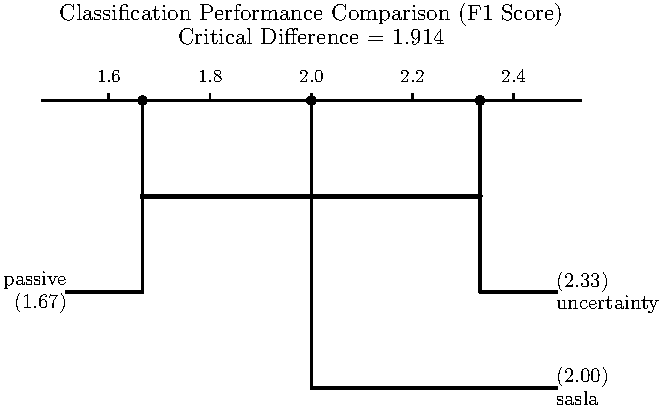
\includegraphics[width=\linewidth]{plots/classification_critical_difference.pdf}
		\caption{Critical difference plot for the average ranks of the learning algorithms performance for the classification problems}
		\label{fig:classification_cd}
	\end{figure}
	
	Figure~\ref{fig:classification_cd} shows that the SASLA algorithm ranked lower than the uncertainty sampling algorithm for the classification problems. Figure~\ref{fig:regression_cd}, however, shows that the uncertainty sampling algorithm ranked lower than SASLA for the regression problems. This suggests that the SASLA algorithm should be considered over the uncertainty sampling algorithm for classification problems and uncertainty sampling should be considered for regression problems over the SASLA algorithm. 
	
	\begin{figure}[htbp]
		\centering
		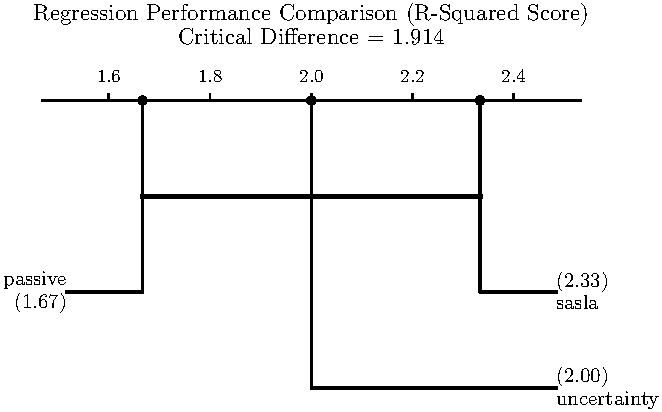
\includegraphics[width=\linewidth]{plots/regression_critical_difference.pdf}
		\caption{Critical difference plot for the average ranks of the learning algorithms performance for the regression problems}
		\label{fig:regression_cd}
	\end{figure}
	
	The results in Tables~\ref{tab:classification_wtl} and \ref{tab:regression_wtl} represent the number of classification and regression datasets on which the uncertainty sampling and SASLA algorithms win, tie or lose compared to the passive learning baseline. These results were calculated by conducting a pairwise comparison using paired t-tests for every performance metric of each problem. A win or loss is assigned if an algorithm performed significantly better or worse than the baseline, otherwise a tie is assigned for no significant difference. The results in Table~\ref{tab:classification_wtl} represent the classification wins, ties and losses. The uncertainty sampling algorithm performed significantly better than passive learning on one of the classification datasets and tied on the rest. The SASLA algorithm tied with the passive learning algorithm on all classification datasets.
	
	\begin{table}[htbp]
		\centering
		\caption{The number of classification datasets on which uncertainty sampling and SASLA significantly Win (W), Tie (T), or Lose (L) compared to the passive learning baseline}
		\label{tab:classification_wtl}
		\begin{tabular}{lcccc}
			\hline
			& \textbf{Accuracy} & \textbf{F1 Score} & \textbf{Precision} & \textbf{Recall} \\
			\hline
			\textbf{Algorithm} & \textbf{W/T/L} & \textbf{W/T/L} &\textbf{W/T/L} & \textbf{W/T/L} \\
			\hline
			Uncertainty & 1/2/0 & 1/2/0 & 1/2/0 & 1/2/0 \\
			SASLA       & 0/3/0 & 0/3/0 & 0/3/0 & 0/3/0 \\
			\hline
		\end{tabular}
	\end{table}
	
	Neither the uncertainty sampling or SASLA algorithms won against the passive learning baseline for the regression problems. The uncertainty sampling algorithm lost twice for and drew once. The SASLA algorithm drew twice and lost once. 
	
	\begin{table}[htbp]
		\centering
		\caption{The number of regression datasets on which uncertainty sampling and SASLA significantly Win, Tie, or Lose compared to the passive learning baseline}
		\label{tab:regression_wtl}
		\begin{tabular}{lcccc}
			\hline
			& \textbf{R-squared} & \textbf{MAE} & \textbf{MSE} & \textbf{RMSE} \\
			\hline
			\textbf{Algorithm} & \textbf{W/T/L} & \textbf{W/T/L} &\textbf{W/T/L} & \textbf{W/T/L} \\
			\hline
			Uncertainty & 0/1/2 & 0/1/2 & 0/1/2 & 0/1/2 \\
			SASLA       & 0/2/1 & 0/2/1 & 0/2/1 & 0/2/1 \\
			\hline
		\end{tabular}
	\end{table}
	
	The results from the non-parametric statistical tests showed that there were no significant differences between the performances of the three algorithms. The parametric pairwise comparison t-tests, however, were able to identify significant differences between the baseline passive learning and the uncertainty sampling and SASLA algorithms in the forms of wins, losses and ties. The results from both statistical tests agree that the passive learning algorithm was overall the better performing algorithm. The passive learning algorithm had the lowest ranks in both critical difference plots and only lost once in the pairwise comparison t-tests. 
	
	\section{Conclusion}\label{C}
	This assignment evaluated the performance of passive learning, uncertainty sampling and SASLA across multiple classification and regression problems of varying complexity. The results demonstrated that there was no single algorithm that consistently outperformed the others across all datasets. The benefits for each approach were determined to be problem dependent.
	
	All three learning algorithms achieved competitive performance for the classification problems. Uncertainty sampling and SASLA occasionally outperformed passive learning on certain datasets. The statistical tests however concluded that there was no statistically significant difference between the algorithms. For the regression tasks, passive learning provided more consistent perform across the varying complexity of problems where methods such as uncertainty sampling struggled with the more complex problems. SASLA proved capable of generating competitive performance for all problems, however did not demonstrate a clear advantage over passive learning where its pattern selection mechanism required larger subsets of data for more complex problems. 
	
	The statistical tests confirmed that the observed performance differences were not significant. Non-parametric tests indicated that no algorithm clearly performed better than the other algorithms. The pairwise comparisons highlighted wins and losses for uncertainty sampling and SASLA against the baseline passive learning. The results from these comparisons were mostly in favour of passive learning algorithm.
	
	The active learning strategies such as uncertainty sampling and SASLA have potential to offer advantages in certain cases, however they do not guarantee consistent improvements over the passive learning baseline.
	
	\begin{thebibliography}{00}
		\bibitem{github} KellenMossner, ``Assignment-3,'' \textit{GitHub}, 2025. [Online]. Available: https://github.com/KellenMossner/MachineLearning441/tree/main/Assignment-3. [Accessed: Oct. 1, 2025].
		\bibitem{lewis1994sequential} D.~D.~Lewis and W.~A.~Gale, ``A sequential algorithm for training text classifiers,'' in \emph{Proc. 17th Annual Int. ACM SIGIR Conf. on Research and Development in Information Retrieval}, New York, NY, USA: Springer-Verlag, 1994, pp. 3--12.
		\bibitem{lakshminarayanan2017} B.~Lakshminarayanan, A.~Pritzel, and C.~Blundell, ``Simple and scalable predictive uncertainty estimation using deep ensembles,'' \emph{arXiv preprint arXiv:1612.01474}, 2017. [Online]. Available: https://arxiv.org/abs/1612.01474
		\bibitem{sharma2017} M. Sharma and M. Bilgic, ``Evidence-based uncertainty sampling for active learning,'' \emph{Data Mining and Knowledge Discovery}, vol.~31, no.~1, pp.~164--202, Jan. 2017, doi: 10.1007/s10618-016-0460-3.
		\bibitem{engelbrecht2001} A. Engelbrecht, ``Sensitivity analysis for selective learning by feedforward neural networks,'' \emph{Fundamenta Informaticae}, vol.~45, pp.~295--328, Aug. 2001, doi: 10.3233/FUN-2001-45402.
		\bibitem{breast} W. Wolberg, O. Mangasarian, N. Street, and W. Street. "Breast Cancer Wisconsin (Diagnostic)," UCI Machine Learning Repository, 1993. [Online]. Available: https://doi.org/10.24432/C5DW2B.
		\bibitem{mobile} I. Abhishek, ``Mobile Price Classification,'' Kaggle, 2017. [Online]. Available: https://www.kaggle.com/datasets/iabhishekofficial/mobile-price-classification
		\bibitem{letter} D. Slate. "Letter Recognition," UCI Machine Learning Repository, 1991. [Online]. Available: https://doi.org/10.24432/C5ZP40.
		\bibitem{boston} D. Harrison and D. L. Rubinfeld, ``Hedonic prices and the demand for clean air,'' \emph{Journal of Environmental Economics and Management}, vol.~5, pp.~81--102, 1978.
		\bibitem{concrete} I. Yeh. "Concrete Compressive Strength," UCI Machine Learning Repository, 1998. [Online]. Available: https://doi.org/10.24432/C5PK67.
		\bibitem{abalone} W. Nash, T. Sellers, S. Talbot, A. Cawthorn, and W. Ford. "Abalone," UCI Machine Learning Repository, 1994. [Online]. Available: https://doi.org/10.24432/C55C7W.
		\bibitem{paszke2019pytorch}	A. Paszke, S. Gross, F. Massa, A. Lerer, J. Bradbury, G. Chanan, T. Killeen, Z. Lin, N. Gimelshein, L. Antiga, A. Desmaison, A. Kopf, E. Yang, Z. DeVito, M. Raison, A. Tejani, S. Chilamkurthy, G. Tang, Y. Li, M. Wong, J. Auer, D. Auer, B. Yu, A. Li, K. Xu, and S. Chintala, ``PyTorch: An Imperative Style, High-Performance Deep Learning Library,'' in \textit{Advances in Neural Information Processing Systems 32}, 2019, pp. 8024--8035.
	\end{thebibliography}
	
\end{document}